% Drawing 146/04-5 -- folder 146, batch 04, archive page 63 (PDF page 64).
% Transcription: Dans la moitié inférieure : un petit triangle hachuré ; un icosaèdre en perspective dont les arêtes portent les lettres $a, b, c, d, e$ ; un grand patron déplié de faces (pentagones et quadrilatères) aux arêtes marquées $a, \ldots, e$, avec des flèches courbes indiquant des recollements ; à droite, trois sphères au crayon portant des points cerclés et des méridiens.
% Kind: polyhedron net (pentagons and quadrilaterals), icosahedron sketch, spheres. Method 2 (schematic redraw from the facsimile). Status: partial.
% Notes: Redrawn stroke by stroke on computed vertices: every stroke of the net and of the small icosahedron is drawn between named vertices shared by the strokes that meet there. Icosahedron sketch (top left): the top spike, the outer and inner top vertices, the left, right and bottom vertices and the strokes between them as he drew them, the dots on the edges placed on those edges, the crosses at the left, and his edge letters a-e where they can be read. Small hatched triangle at the top, with the two faint strokes near it (pencil). The net: the central pentagon (sides a, d, e, b and the doubled left side), the inner vertex joined to the bottom right vertex, to the letter in the middle and up to the right (e); on the left the quadrilaterals (b, a, d, d, e), above them the faces through e, b (dotted) and d, the long faint vertical to the top of the pentagon and the faint strokes on the left (pencil), on the right the strokes towards a vertex beyond the crop edge (a, c); the five curved gluing arrows and the dotted one; the edge letters as they stand. Three pencil spheres at the right with their ringed points on the equators (projected) and meridians ending at the poles; the lowest has the bold axis and the dashed meridian. Not encoded: the net is faint and overdrawn, so which edges are glued cannot be fixed from the figure alone. Still differs: the faces of the net are a reading of overdrawn pencil (his doubled strokes drawn once, some faint strokes beyond the drawn vertices left out); the heavy letter in the middle of the net (« S » or « 5 »?) and the faint erased letters inside the pentagon are left out; the letters on the icosahedron are placed as read, some uncertain. Redrawn 2026-11-09 (issue 128): to check again. 2026-11-13, Claude Opus 5.5, overlay check (issue 147): rasterised from its own coordinates over the 400 dpi colour scan (250 ppi native) on a unit grid; the small icosahedron, the hatched triangle, the faces of the net with their letters and gluing arrows, and the three pencil spheres lie on their ink to within 1 to 2 units where the faint pencil can be followed, so the redraw is unchanged. Not compiled (no TeX in the session). Still differs, as before: the faces of the net are a reading of overdrawn pencil (doubled strokes drawn once, some faint strokes beyond the drawn vertices left out); the heavy letter in the middle of the net and the faint erased letters in the pentagon are left out; some letters on the icosahedron are uncertain.
% Coordinates: 1 unit = 1 mm = 1/100 of the crop width (bbox in page fractions: [0.11, 0.44, 0.88, 0.84]).
% Redrawn by Claude (claude-opus-5-5), issue #73, 2026-11-09; not checked by a human; not compiled (no TeX in the session).
% Checked by Claude (claude-opus-5-5) 2026-11-13 (issue #147): overlaid on the 400 dpi colour facsimile; not compiled (no TeX in the session). Not checked by a human. Status: partial.
% Rights: reproduces part of the work -- behind RENDER_TRANSCRIPTS, never published by itself.
\documentclass[tikz,border=3pt]{standalone}
\usepackage{amsmath,amssymb}
\usetikzlibrary{patterns,arrows.meta}
\tikzset{pencil/.style={black!45}, struck/.style={black!35}, mark/.style={circle,draw,inner sep=1.3pt}, pt/.style={circle,fill,inner sep=0.9pt}, opt/.style={circle,draw,fill=white,inner sep=1.1pt}}
\begin{document}
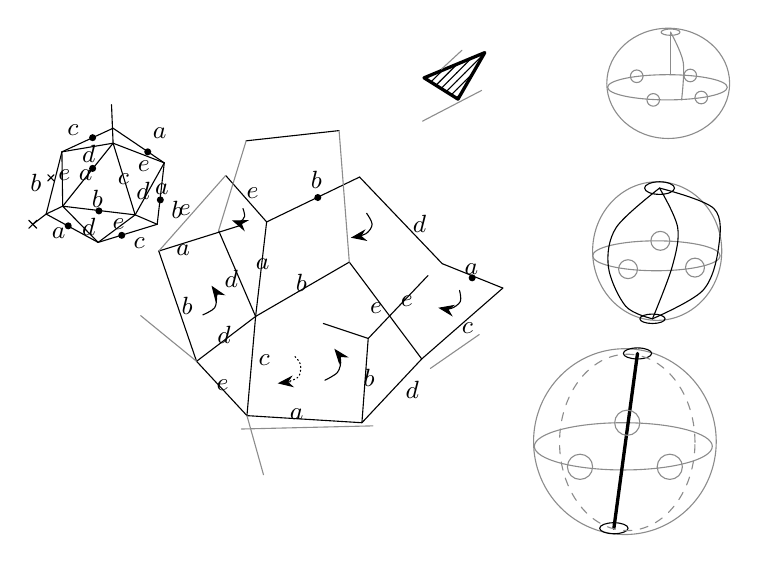
\begin{tikzpicture}[x=1mm,y=1mm,line cap=round,line join=round,font=\scriptsize]
\draw (13.3,-9.4) -- (13.5,-14.3);
\draw (7,-15.4) -- (13.5,-12.4);
\draw (7,-15.4) -- (13.5,-14.3);
\draw (13.5,-12.4) -- (20,-16.8);
\draw (13.5,-14.3) -- (20,-16.8);
\draw (7,-15.4) -- (7.1,-22.3);
\draw (7,-15.4) -- (5,-23.3);
\draw (7.1,-22.3) -- (13.5,-14.3);
\draw (7.1,-22.3) -- (16.3,-23.4);
\draw (13.5,-14.3) -- (16.3,-23.4);
\draw (16.3,-23.4) -- (20,-16.8);
\draw (20,-16.8) -- (19.1,-24.6);
\draw (7.1,-22.3) -- (5,-23.3);
\draw (5,-23.3) -- (3.3,-24.6);
\draw (5,-23.3) -- (11.6,-26.9);
\draw (7.1,-22.3) -- (11.6,-26.9);
\draw (16.3,-23.4) -- (11.6,-26.9);
\draw (16.3,-23.4) -- (19.1,-24.6);
\draw (11.6,-26.9) -- (19.1,-24.6);
\draw (2.8,-24.1) -- (3.8,-25.1);
\draw (2.8,-25.1) -- (3.8,-24.1);
\draw (5.2,-18.3) -- (6,-19.1);
\draw (5.2,-19.1) -- (6,-18.3);
\node[pt] at (10.9,-13.6) {};
\node[pt] at (17.9,-15.4) {};
\node[pt] at (10.9,-17.5) {};
\node[pt] at (11.7,-22.9) {};
\node[pt] at (19.5,-21.5) {};
\node[pt] at (7.8,-24.8) {};
\node[pt] at (14.6,-26) {};
\node[inner sep=1pt] at (8.4,-12.6) {\small $c$};
\node[inner sep=1pt] at (19.4,-13) {\small $a$};
\node[inner sep=1pt] at (10.4,-15.6) {\small $d$};
\node[inner sep=1pt] at (17.4,-17.2) {\small $e$};
\node[inner sep=1pt] at (3.7,-19.3) {\small $b$};
\node[inner sep=1pt] at (7.3,-18.4) {\small $e$};
\node[inner sep=1pt] at (10,-18.3) {\small $a$};
\node[inner sep=1pt] at (14.8,-18.9) {\small $c$};
\node[inner sep=1pt] at (11.5,-21.4) {\small $b$};
\node[inner sep=1pt] at (17.3,-20.4) {\small $d$};
\node[inner sep=1pt] at (19.7,-20.1) {\small $a$};
\node[inner sep=1pt] at (21.6,-22.8) {\small $b$};
\node[inner sep=1pt] at (22.6,-22.8) {\small $e$};
\node[inner sep=1pt] at (6.6,-25.7) {\small $a$};
\node[inner sep=1pt] at (10.4,-24.9) {\small $d$};
\node[inner sep=1pt] at (14.2,-24.6) {\small $e$};
\node[inner sep=1pt] at (16.8,-27) {\small $c$};
\draw[very thick] (53,-6) -- (60.7,-2.8) -- (57.3,-8.7) -- cycle;
\fill[pattern=north east lines] (53,-6) -- (60.7,-2.8) -- (57.3,-8.7) -- cycle;
\draw[pencil] (52.8,-11.5) -- (60.3,-7.6);
\draw[pencil] (55.2,-4.9) -- (57.8,-2.5);
\draw (30.5,-48.9) -- (45.1,-49.8);
\draw (45.1,-49.8) -- (52.7,-41.7);
\draw (52.7,-41.7) -- (43.5,-29.4);
\draw (43.5,-29.4) -- (31.6,-36.3);
\draw (31.6,-36.3) -- (30.5,-48.9);
\draw (45.9,-39.1) -- (45.1,-49.8);
\draw (45.9,-39.1) -- (40.2,-37.2);
\draw (45.9,-39.1) -- (53.5,-31.1);
\draw (19.3,-28) -- (24.1,-42);
\draw (24.1,-42) -- (30.5,-48.9);
\draw (31.6,-36.3) -- (24.1,-42);
\draw (26.9,-25.4) -- (31.6,-36.3);
\draw (19.3,-28) -- (29.5,-24.8);
\draw (27.8,-18.4) -- (33,-24.3);
\draw (33,-24.3) -- (44.8,-18.6);
\draw (44.8,-18.6) -- (55.3,-29.6);
\draw (33,-24.3) -- (31.6,-36.3);
\draw (55.3,-29.6) -- (63,-32.7);
\draw (52.7,-41.7) -- (63,-32.7);
\draw (30.4,-14) -- (42.2,-12.7);
\draw[pencil] (19.3,-28) -- (27.8,-18.4);
\draw[pencil] (42.2,-12.7) -- (43.5,-29.4);
\draw[pencil] (30.4,-14) -- (26.9,-25.4);
\draw[pencil] (17,-36.2) -- (24.1,-42);
\draw[pencil] (30.5,-48.9) -- (32.6,-56.4);
\draw[pencil] (29.8,-50.6) -- (46.5,-50.2);
\draw[pencil] (53.8,-42.9) -- (60,-38.6);
\node[pt] at (39.5,-21.2) {};
\node[pt] at (59.1,-31.4) {};
\draw[-{Stealth[length=2mm]}] plot[smooth, tension=0.55] coordinates {(30,-22.6) (30.2,-23.6) (29.6,-24.3) (28.6,-24.1)};
\draw[-{Stealth[length=2mm]}] plot[smooth, tension=0.55] coordinates {(45.7,-23.2) (46.4,-24.6) (45.6,-25.8) (43.7,-26.3)};
\draw[-{Stealth[length=2mm]}] plot[smooth, tension=0.55] coordinates {(57.5,-33) (57.6,-34.4) (56.4,-35.3) (54.8,-35.2)};
\draw[-{Stealth[length=2mm]}] plot[smooth, tension=0.55] coordinates {(24.9,-36.1) (26.4,-35.2) (26.6,-33.6) (26,-32.4)};
\draw[-{Stealth[length=2mm]}] plot[smooth, tension=0.55] coordinates {(40.4,-44.4) (42,-43.4) (42.4,-41.8) (41.6,-40.4)};
\draw[densely dotted] plot[smooth, tension=0.55] coordinates {(36.6,-41.4) (37.3,-42.4) (37.1,-43.9) (36,-44.5)};
\draw[-{Stealth[length=2mm]}] (36,-44.6) -- (34.4,-44.8);
\node[inner sep=1pt] at (22.4,-27.9) {\small $a$};
\node[inner sep=1pt] at (22.9,-35) {\small $b$};
\node[inner sep=1pt] at (28.5,-31.5) {\small $d$};
\node[inner sep=1pt] at (27.6,-38.6) {\small $d$};
\node[inner sep=1pt] at (27.4,-45) {\small $e$};
\node[inner sep=1pt] at (32.7,-41.9) {\small $c$};
\node[inner sep=1pt] at (32.5,-29.7) {\small $a$};
\node[inner sep=1pt] at (31.2,-20.6) {\small $e$};
\node[inner sep=1pt] at (39.3,-19) {\small $b$};
\node[inner sep=1pt] at (52.4,-24.6) {\small $d$};
\node[inner sep=1pt] at (37.4,-32) {\small $b$};
\node[inner sep=1pt] at (46.9,-35.2) {\small $e$};
\node[inner sep=1pt] at (50.8,-34.3) {\small $e$};
\node[inner sep=1pt] at (46,-44.1) {\small $b$};
\node[inner sep=1pt] at (51.5,-45.6) {\small $d$};
\node[inner sep=1pt] at (36.8,-48.7) {\small $a$};
\node[inner sep=1pt] at (58.5,-37.8) {\small $c$};
\node[inner sep=1pt] at (59,-30.3) {\small $a$};
\draw[pencil] (84,-6.7) ellipse[x radius=7.8, y radius=7];
\draw[pencil] (83.9,-7.2) ellipse[x radius=7.6, y radius=1.6];
\draw[pencil] (84.3,-0.2) -- (84.3,-5.6);
\draw[pencil] plot[smooth, tension=0.55] coordinates {(84.3,-0.2) (85.9,-4) (85.7,-8.8)};
\draw[pencil] (80,-5.8) circle[radius=0.8];
\draw[pencil] (86.8,-5.7) circle[radius=0.8];
\draw[pencil] (82.1,-8.8) circle[radius=0.8];
\draw[pencil] (88.2,-8.5) circle[radius=0.8];
\draw[pencil] (84.3,-0.2) ellipse[x radius=1.2, y radius=0.4];
\draw[pencil] (82.6,-28) ellipse[x radius=8.2, y radius=8.8];
\draw[pencil] (82.5,-28.6) ellipse[x radius=8.1, y radius=1.9];
\draw (82.9,-20) ellipse[x radius=1.9, y radius=0.8];
\draw (82,-36.6) ellipse[x radius=1.6, y radius=0.6];
\draw plot[smooth, tension=0.55] coordinates {(82.9,-20) (77.4,-25) (76.4,-30) (78.6,-35) (82,-36.6)};
\draw plot[smooth, tension=0.55] coordinates {(82.9,-20) (89.8,-22.6) (90.4,-27.5) (88.4,-33) (82,-36.6)};
\draw plot[smooth, tension=0.55] coordinates {(82.9,-20) (85.2,-25) (84.5,-30) (82,-36.6)};
\draw[pencil] (83,-26.7) circle[radius=1.2];
\draw[pencil] (78.9,-30.3) circle[radius=1.2];
\draw[pencil] (87.4,-30.1) circle[radius=1.2];
\draw[pencil] (78.5,-52.2) ellipse[x radius=11.6, y radius=11.8];
\draw[pencil] (78.3,-52.8) ellipse[x radius=11.3, y radius=3];
\draw (80.1,-41) ellipse[x radius=1.8, y radius=0.7];
\draw (77.1,-63.2) ellipse[x radius=1.8, y radius=0.7];
\draw[very thick] (80.1,-41) -- (77.1,-63.2);
\draw[dashed,pencil] (78.8,-52.3) ellipse[x radius=8.6, y radius=11.2];
\draw[pencil] (78.8,-49.8) circle[radius=1.6];
\draw[pencil] (72.8,-55.4) circle[radius=1.6];
\draw[pencil] (84.2,-55.4) circle[radius=1.6];
\end{tikzpicture}
\end{document}
